\documentclass[11pt]{article}

% Paquetes
%===================================================================================================

% Establecemos los márgenes
\usepackage[a4paper, margin=1in]{geometry}

% Separacion entre parrafos
\setlength{\parskip}{1em}

% Paquete para incluir codigo
\usepackage{listings}

% Paquete para incluir imagenes
\usepackage{graphicx}
\graphicspath{ {./Imagenes/} }

% Para fijar las imagenes en la posicion deseada
\usepackage{float}

% Para que el codigo acepte caracteres en utf8
\lstset{literate=
  {á}{{\'a}}1 {é}{{\'e}}1 {í}{{\'i}}1 {ó}{{\'o}}1 {ú}{{\'u}}1
  {Á}{{\'A}}1 {É}{{\'E}}1 {Í}{{\'I}}1 {Ó}{{\'O}}1 {Ú}{{\'U}}1
  {à}{{\`a}}1 {è}{{\`e}}1 {ì}{{\`i}}1 {ò}{{\`o}}1 {ù}{{\`u}}1
  {À}{{\`A}}1 {È}{{\'E}}1 {Ì}{{\`I}}1 {Ò}{{\`O}}1 {Ù}{{\`U}}1
  {ä}{{\"a}}1 {ë}{{\"e}}1 {ï}{{\"i}}1 {ö}{{\"o}}1 {ü}{{\"u}}1
  {Ä}{{\"A}}1 {Ë}{{\"E}}1 {Ï}{{\"I}}1 {Ö}{{\"O}}1 {Ü}{{\"U}}1
  {â}{{\^a}}1 {ê}{{\^e}}1 {î}{{\^i}}1 {ô}{{\^o}}1 {û}{{\^u}}1
  {Â}{{\^A}}1 {Ê}{{\^E}}1 {Î}{{\^I}}1 {Ô}{{\^O}}1 {Û}{{\^U}}1
  {ã}{{\~a}}1 {ẽ}{{\~e}}1 {ĩ}{{\~i}}1 {õ}{{\~o}}1 {ũ}{{\~u}}1
  {Ã}{{\~A}}1 {Ẽ}{{\~E}}1 {Ĩ}{{\~I}}1 {Õ}{{\~O}}1 {Ũ}{{\~U}}1
  {œ}{{\oe}}1 {Œ}{{\OE}}1 {æ}{{\ae}}1 {Æ}{{\AE}}1 {ß}{{\ss}}1
  {ű}{{\H{u}}}1 {Ű}{{\H{U}}}1 {ő}{{\H{o}}}1 {Ő}{{\H{O}}}1
  {ç}{{\c c}}1 {Ç}{{\c C}}1 {ø}{{\o}}1 {å}{{\r a}}1 {Å}{{\r A}}1
  {€}{{\euro}}1 {£}{{\pounds}}1 {«}{{\guillemotleft}}1
  {»}{{\guillemotright}}1 {ñ}{{\~n}}1 {Ñ}{{\~N}}1 {¿}{{?`}}1 {¡}{{!`}}1
}

% Para que no se salgan las lineas de codigo
% Para fijar una fuente que resalte
\lstset{breaklines=true, basicstyle=\ttfamily}


% Para que los metadatos que escribe latex esten en español
\usepackage[spanish]{babel}
\decimalpoint % Para que no se cambie el punto a la coma

% Para la bibliografia
% Sin esto, los enlaces de la bibliografia dan un error de compilacion
\usepackage{url}

% Para enlaces clickables
\usepackage{hyperref}

% Para mostrar graficas de dos imagenes, cada una con su caption, y con un caption comun
\usepackage{subcaption}

% Simbolo de los numeros reales
\usepackage{amssymb}

% Para que los codigos tengan una fuente distinta
\usepackage{courier}

\lstdefinestyle{CustomStyle}{
  language=Python,
  numbers=left,
  stepnumber=1,
  numbersep=10pt,
  tabsize=4,
  showspaces=false,
  showstringspaces=false
  basicstyle=\tiny\ttfamily,
}

% Para incluir tablas en csv
\usepackage{csvsimple}

% Para referenciar secciones usando el nombre de las secciones
\usepackage{nameref}

% Para enumerados dentro de enumerados
\usepackage{enumitem}

% Para mejores tablas
\usepackage{tabularx}

% Para poder tener el mismo identificador en dos tablas separadas
\usepackage{caption}

% Mostrar la página de las referencias en el indice del documento
\usepackage[nottoc,numbib]{tocbibind}

% Para mostrar las matrices
\usepackage{amsmath}

% Metadatos del documento
%===================================================================================================
\title{
    {Metaheurísticas - Proyecto Final}\\
    {\emph{Battle Royale Metaheuristic}}\\
    {\emph{Cec17 Competition}}
}

\author{
    {Sergio Quijano Rey - 72103503k}\\
    {sergioquijano@correo.ugr.es} \\
    {4º Doble Grado Ingeniería Informática y Matemáticas}
}

\date{\today}

% Separacion entre parrafos
\setlength{\parskip}{1em}

% Contenido del documento
%===================================================================================================
\begin{document}

% Portada del documento
\maketitle
\pagebreak

% Indice de contenidos
\tableofcontents

% Lista de figuras
\listoffigures

% Lista de tablas
\listoftables

\pagebreak
\section{Identificación del problema a resolver}

El problema a resolver consiste en realizar una propuesta de metaheurística original para problemas de codificación real. A partir de esta propuesta, realizaremos una implementación de dicha metaheurística original, y trabajaremos la competición \emph{Cec17}.

Para trabajar con dicha competición, usaremos el \emph{software} desarrollado por Daniel Molina, que se encuentra en \cite{daniel_repo:online}. En dicho repositorio encontramos el siguiente \emph{software}:

\begin{itemize}
    \item Librería escrita en \lstinline{C} que define las 31 funciones de \emph{fitness} que debemos optimizar, para las distintas dimensiones disponibles, así como otras funcionalidades
    \item Código \lstinline{python} para generar unas tablas \emph{Excel} que poder usar en \href{tacolab.org} para comparar con otros algoritmos de referencia
    \item Wrapper para \lstinline{Python}, con el que podemos acceder a todas las funciones definidas en la ya mencionada librería dinámica
\end{itemize}

En nuestro caso, como indicaron los profesores de la asignatura, por problemas con los tiempos de cómputo, trabajaremos con dimensión 10 y 30. Además, repetiremos por cada función y por cada dimensión, 10 ejecuciones distintas.

Por tanto, usamos un \emph{fork} de este repositorío para desarrollar nuestro trabajo, que se encuentra en \cite{repositorio:online}.

\pagebreak
\section{Descripción de la metaheurística}

\subsection{Propuesta original}

La metaheurística se basa en un género de videojuegos conocido como \emph{Battle Royale}. La dinámica de estos videojuegos se inspiran fuertemente en la serie de libros y posteriores películas `\emph{Los juegos del Hambre}', por lo que si el lector está familiarizado con estas novelas le será fácil seguir la siguiente explicación:

Una serie de jugadores (entre 50 y 100) se reparten a lo largo de un mapa. El objetivo es ser el último jugador vivo durante la partida. Para ello, tienen que seguir una serie de dinámicas durante la partida:

En primer lugar, al principio de la partida, los jugadores deben recolectar armas y otros recursos, porque todos los jugadores aparecen en el mapa sin equipación alguna. Esto puede verse reflejado en la metaheurística como una primera búsqueda local, muy suave, aplicada a las soluciones iniciales aleatorias

En segundo lugar, los jugadores deben matar y defenderse de los otros jugadores con los que se pueden encontrar a través del mapa. Para reflejar esto, si dos soluciones están muy cerca la una de la otra, estas dos soluciones compiten entre sí. El mejor jugador, que está mejor equipado, tiene una probabilidad alta de ganar la pelea, matando al otro jugador. Sin embargo, el peor jugador tiene una probabilidad pequeña de matar al mejor jugador (en el juego, puedes ir mejor equipado, pero perder el duelo por ser un jugador menos habilidoso). Soluciones muy cerca en el sentido en el que cierta distancia de los vectores que representan las dos soluciones estén por debajo de un valor dado.

En tercer lugar, a partir de cierto tiempo, el mapa se cierra incrementalmente sobre un área circular del mapa, cada vez más pequeña. Con esto se fomenta que los jugadores tengan que enfrentarse unos con otros, y potenciando que los jugadores mejor equipados y más habilidosos ganen sin tener que esperar demasiado tiempo a malos jugadores escondidos por el mapa.

Para representar esto en la metaheurística, a partir de cierta iteración, se realizarán eliminaciones de la población. A partir de este momento, cada cierto número de iteraciones, los $\lambda$ peores elementos de la población, son eliminados al quedar fuera del círculo

La siguiente imagen, extraída de \cite{other_paper:paper}, ilustra de forma clara cuál es la mecánica del cierre del círculo:

\begin{figure}[H]
    \centering
    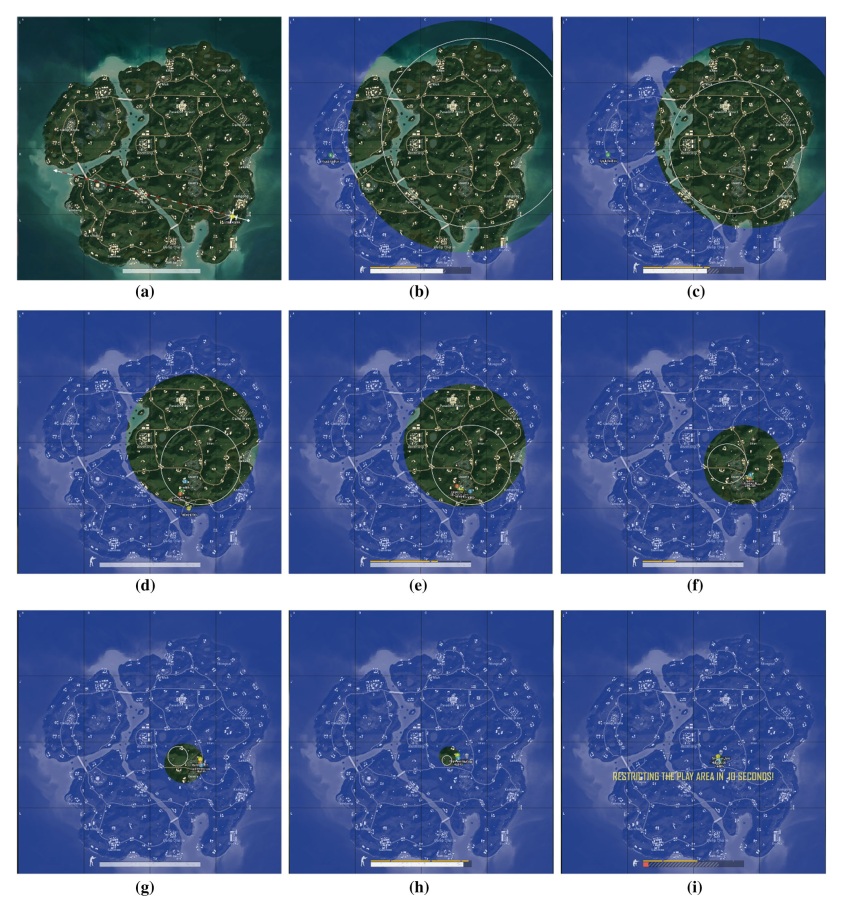
\includegraphics[width=0.6\textwidth]{cierre_circulo}
    \caption{Ilustración de la mecánica del cierre del círculo}
\end{figure}

En cuarto lugar, hay una cierta probabilidad de revivir si un jugador muere, aunque no es muy alta. Cuando un jugador revive, reaparece sin nada de lo que habías estado recolectando durante la partida. Se otorga un periodo de inmunidad en el que el jugador que ha revivido tiene que recolectar rápidamente recursos para ser competitivo contra jugadores que van más avanzados en la partida. Además, puede ser que reaparezcan fuera del círculo, luego deben lograr entrar al círculo en el tiempo de gracia

Por tanto, si un jugador muere, tiene una probabilidad dada (potencialmente baja) de revivir. Al revivir, pierde todos sus recursos. Esto se materializa en que se le asigna una solución aleatoria. En nomenclatura de nuestra metaheurística, reaparece en una posición aleatoria. Además, el periodo de gracia se materializa en que dispondrá de un número de iteraciones de una búsqueda local suave,  para intentar ser competitivo con el resto de soluciones que llevan toda la partida mejorando su fitness.

Decidimos también que, si un jugador muere contra el mejor jugador hasta el momento, revive siempre. Esto no se aplica cuando quedan menos de un número dado de jugadores (fase final de la partida)

Además de esto, consideramos algunos aspectos generales a todas las metaheurísticas vistas en clase:

En las distintas iteraciones, realizaremos una búsqueda local suave sobre las soluciones (para representar el movimiento por el mapa de los jugadores en la partida). Y como es habitual, partiremos de una población inicial aleatoria de jugadores. En el propio juego, los jugadores saltan desde el cielo eligiendo la posición inicial, y por tanto, podemos modelar este comportamiento como aleatorio.

\subsection{Modificaciones a la propuesta original}

Como era de esperar, esta propuesta original debe ser modificada ligeramente, pues algunas decisiones a nivel de ingeniería tienen más sentido. Las modificaciones que hemos considerado tras experimentar con la implementación de la metaheurística (implementación que se desarrollará en \emph{\ref{implementacion}. \nameref{implementacion}}) son las siguientes:

\begin{itemize}
    \item En un principio habíamos pensado en emplear la distancia euclídea para comprobar si dos jugadores estaban demasiado cerca. Sin embago, acabamos usando la distancia Manhattan porque es más rápida de computar. Esta distancia viene dada por $$\sum |w_i|$$ donde los coeficientes se definen como $$w := jugador_1 - jugador_2$$
    \item La mecánica de eliminar a los $\lambda$ peores jugadores en cada iteración, a partir de cierto momento, provoca que perdamos mucha variedad en la población prematuramente. En vez de eso, definimos un porcentaje que, a partir de un valor del radio del círculo $r$ por encima de $1.0$, que va descendiendo iteración tras iteración hasta llegar a $r = 1.0$. En cada iteración se eliminan los jugadores con \emph{fitness} más de $r$ veces peor que el \emph{fitness} de la mejor solución (recordad que estamos en un problema de minimización de las funciones objetivo)
    \item Tras hacer \emph{parameter tuning} en la sección \emph{\ref{tuning}. \nameref{tuning}}, la probabilidad de revivir acaba siendo 0.5, para nada es una probabilidad baja
    \item Por su poca relevancia, ignoramos la parte en la que comentamos que si un jugador muere contra el mejor jugador, forzosamente revive
\end{itemize}

\pagebreak
\section{Implementación de la metaheurística} \label{implementacion}

El desarrollo de esta metaheurística se ha realizado en \lstinline{python}, debido al rápido desarrollo que permite este lenguaje y la disponibilidad de \emph{wrappers} para el lenguaje gracias a \cite{daniel_repo:online}.

El proceso de instalación y ejecución del software se desarrolla en el \emph{Readme} del repositorio en el que tenemos alojado el código \cite{repositorio:online}, y por tanto no describimos de nuevo este proceso de instalación y ejecución necesario para trabajar con nuestra implementación.

Pasamos a comentar algunos aspectos clave de la implementación (no todo el código en general, que está a nuestro modo de ver lo suficientemente bien documentado como para que sea muy sencillo de leer).

\subsection{Clase \lstinline{Config}}

La clase \lstinline{Config} centraliza todos los parámetros que hemos fijado en nuestra metaheurística. Los atributos estáticos hace que sea fácil acceder a parámetros comunes en distintas partes del código sin una penalización en tiempos de ejecución aparentemente relevante.

Además, como se hace en la función \lstinline{parameter_tuning} de \lstinline{main.py}, podemos modificar estos atributos estáticos para ver cómo afecta esto al rendimiento de nuestra metaheurística.

\subsection{Clase \lstinline{EvalsCounter}}

Esta clase se implementa con el uso del patrón \emph{Singleton}. Su objetivo es centralizar la cuenta de evaluaciones del \emph{fitness} consumidas hasta el momento, sin tener que pasar a todos los métodos una parámetro adicional.

Sin embargo, sospechamos que esto sí que puede introducir una penalización en tiempo de ejecución. Pero al estar escribiendo un primer prototipo, vale más la pena trabajar con un código mas sencillo en el que es más rápido realizar cambios sobre la marcha (como hemos tenido que realizar, al no tener una metaheurística ya desarrollado con un funcionamiento bueno asegurado).

En una versión mejorada en la que los tiempos de ejecución sean más críticos, evitar este patrón \emph{Singleton} es obligado.

\subsection{Clase \lstinline{Player}}

Define un jugador. Principalmente, viene dado por las coordenadas en las que se encuentra, que vienen dadas por \lstinline{self.position}.

Por motivos de eficiencia, \emph{cacheamos} el valor del \emph{fitness}, para evitar desperdiciar evaluaciones del \emph{fitness}. Del mismo modo, en la propia lógica que maneja la cache, usamos el \emph{Singleton} que ya hemos comentado para llevar la cuenta de todas las evaluaciones del \emph{fitness} consumidas.

\subsection{Pseudocódigo del algoritmo}

\subsection{\emph{Parameter Tuning}} \label{tuning}

\pagebreak
\section{Resultados de la metaheurística}

\pagebreak
\section{Hibridación con la búsqueda local \emph{Solis West}}

\pagebreak
\section{Resultados de la hibridación}

\pagebreak
\section{Propuesta de mejoras}

% Evitar el singleton, como ya se ha comentado -> Eficiencia, antipatron, no permite paralelizacion

\pagebreak

% Bibliografia
\bibliography{./References}
\bibliographystyle{acm}

\end{document}
